\documentclass[11pt]{article}

% ====================================================
% ====================================================
% USEPACKAGES AND IMPORTS
% ====================================================
% ====================================================

\usepackage[T1]{fontenc}
\usepackage[utf8]{inputenc}
\usepackage[english]{babel}

\usepackage{fancyhdr}

% definitions
% ====================================================
\let\titleoriginal\title
\renewcommand{\title}[1]{
	\titleoriginal{#1}
	\newcommand{\thetitle}{#1}
}

\setlength{\parskip}{\baselineskip}%
\setlength{\parindent}{0pt}%

% header and footer
\pagestyle{fancy}
\fancyhf{}
\lhead{Applied Machine Learning Fundamentals}
\rhead{\thetitle}
\cfoot{\thepage}

% ====================================================
% ====================================================
% PRESENTATION DATA
% ====================================================
% ====================================================

\title[Decision Trees and Ensembles]{*** Applied Machine Learning Fundamentals *** Decision Trees and Ensembles}
\institute{SAP\,SE}
\author{Daniel Wehner}
\date{\today}
\prefix{DT}

% ====================================================
% ====================================================
% BEGIN OF DOCUMENT
% ====================================================
% ====================================================

\begin{document}

% Title frame
%______________________________________________________________________
\maketitlepage


% Agenda
%______________________________________________________________________
\begin{frame}{Agenda \today}
	\begin{multicols}{2}
		\tableofcontents
	\end{multicols}
\end{frame}


% Section: Introduction
%______________________________________________________________________
\section{Introduction}
\makedivider{Introduction}

% What we want...
\begin{frame}{What we want...}{}
	\divideTwo{0.49}{
		\vspace*{4mm}
		\begin{table}
	\scalebox{0.6}{
	\begin{tabular}{| c | c | c | c | c |}
		\hline
		\highlight{A}	&
		\highlight{F} 	&
		\highlight{S} 	&
		\highlight{N} 	&
		\highlight{H}		\\ \hline\hline
		0	&	1	&	0	&	1	&	1	\\ \hline
		1	&	0	&	0	&	0	&	0	\\ \hline
		1	&	0	&	1	&	0	&	1	\\ \hline
		1	&	1	&	1	&	1	&	0	\\ \hline
		0	&	0	&	1	&	1	&	0	\\ \hline
		0	&	0	&	0	&	1	&	1	\\ \hline
		1	&	0	&	0	&	0	&	0	\\ \hline
		0	&	1	&	0	&	1	&	1	\\ \hline
		1	&	1	&	0	&	0	&	0	\\ \hline
		1	&	0	&	1	&	0	&	1	\\ \hline
		1	&	1	&	1	&	1	&	1	\\ \hline
		1	&	1	&	0	&	1	&	0	\\ \hline
		1	&	0	&	1	&	0	&	0	\\ \hline
		0	&	1	&	0	&	0	&	1	\\ \hline
		1	&	0	&	0	&	1	&	1	\\ \hline
		1	&	1	&	1	&	0	&	0	\\ \hline
	\end{tabular}}
\end{table}
	}{0.49}{
		\input{08_decision_trees/01_tikz/tree}
	}
\end{frame}


% What are Decision Trees?
\begin{frame}{What are Decision Trees?}{}
	\begin{itemize}
		\item Decision trees are induced in a \highlight{supervised} fashion
		\item Originally invented by \textit{Ross Quinlan} (1986)
		\item Decision trees are grown \textbf{recursively} $\rightarrow$ \textit{'divide-and-conquer'}
		\item A decision tree consists of:

		\begin{tabbing}
			\hspace*{2.5cm}\= \kill
			\textbf{Nodes}	\>	Each node corresponds to an attribute test 	\\
			\textbf{Edges}	\>	One edge per possible test outcome			\\
			\textbf{Leaves}	\>	Class label to predict
		\end{tabbing}
	\end{itemize}
\end{frame}


% Classifying new Instances
\begin{frame}{Classifying new Instances}{}
	\divideTwo{0.49}{
		\begin{itemize}
			\item Suppose we get a new instance:
			
			\footnotesize
			\begin{tabbing}
				\hspace*{2.5cm}\= \kill
				\texttt{Outlook}			\>	rainy		\\
				\texttt{Temperature} 		\>	mild	 	\\
				\texttt{Humidity}			\>	normal	\\
				\texttt{Wind}			\>	strong
			\end{tabbing}
			\normalsize

			\item \textbf{What is its class?}
			\item Answer: \textbf{No}
		\end{itemize}
	}{0.49}{
		\input{08_decision_trees/01_tikz/tree}
	}
\end{frame}


% Another Decision Tree...
\begin{frame}{Another Decision Tree...}{}
	\bubble{1}{11}{\footnotesize \textbf{Is this one better?}}
	\vspace*{-2mm}
	% Set the overall layout of the tree
\tikzstyle{level 1}=[level distance=2cm,sibling distance=6cm]
\tikzstyle{level 2}=[level distance=2.5cm,sibling distance=2cm]
\tikzstyle{level 3}=[level distance=2.5cm,sibling distance=1.5cm]

% Define styles for bags and leafs
\tikzstyle{bag}=[rectangle,draw=black,text width=4em,text centered]
\tikzstyle{end}=[circle,draw=black,minimum width=3pt,fill,inner sep=0pt]

\begin{figure}
	\centering
	\begin{tikzpicture}[
		scale=0.6,
		every node/.style={scale=0.5},
		sloped
	]
		\node[bag]{\highlight{Temp.}}
    		child{
     	   		node[bag]{\highlight{Outlook}}        
            			child{
                			node[end, label=below:{\textbf{\underline{No}}}]{}
                			edge from parent
                			node[above]{\textit{sunny}}
            			}
            			child{
                			node[end, label=below:{\textbf{\textcolor{red}{\underline{?}}}}]{}
               			edge from parent
                			node[above]{\textit{rain}}
            			}
				child{
                			node[end, label=below:{\textbf{\underline{Yes}}}]{}
               			edge from parent
                			node[above]{\textit{overcast}}
            			}
            			edge from parent 
            			node[above]{\textit{hot}}
    		}
		child{
        		node[bag]{\highlight{Outlook}}        
        		child {
                		node[bag]{\highlight{Humid.}}
                		child{
                			node[end, label=below:{\textbf{\underline{No}}}]{}
                			edge from parent
                			node[above]{\textit{high}}
                		}
				child{
                			node[end, label=below:{\textbf{\underline{Yes}}}]{}
                			edge from parent
                			node[above]{\textit{normal}}
                		}
				child[missing]{}
                		edge from parent
                		node[above]{\textit{sunny}}
            		}
            		child{
                		node[bag]{\highlight{Humid.}}
				child[missing]{}
				child{
					node[bag]{\highlight{Wind}}
					child{
						node[end, label=below:{\textbf{\underline{No}}}]{}
                				edge from parent
                				node[above]{\textit{strong}}
					}
					child{
						node[end, label=below:{\textbf{\underline{Yes}}}]{}
                				edge from parent
                				node[above]{\textit{weak}}
					}
					edge from parent
                			node[above]{\textit{high}}
				}
				child{
					node[end, label=below:{\textbf{\underline{Yes}}}]{}
                			edge from parent
                			node[above]{\textit{normal}}
				}
                		edge from parent
                		node[above]{\textit{rainy}}
            		}
			child{
                		node[end, label=below:{\textbf{\underline{Yes}}}]{}
                		edge from parent
                		node[above]{\textit{overcast}}
            		}
        		edge from parent         
            		node[above]{\textit{mild}}
		}
    		child{
        		node[bag]{\highlight{Outlook}}        
        		child {
                		node[end, label=below:{\textbf{\underline{Yes}}}]{}
                		edge from parent
                		node[above]{\textit{sunny}}
            		}
            		child{
                		node[bag]{\highlight{Humid.}}
                		child{
                			node[end, label=below:{\textbf{\textcolor{red}{\underline{?}}}}]{}
                			edge from parent
                			node[above]{\textit{high}}
                		}
				child{
                			node[bag]{\highlight{Wind}}
					child{
                				node[end, label=below:{\textbf{\underline{No}}}]{}
                				edge from parent
                				node[above]{\textit{strong}}
                			}
					child{
                				node[end, label=below:{\textbf{\underline{Yes}}}]{}
                				edge from parent
                				node[above]{\textit{weak}}
                			}
                			edge from parent
                			node[above]{\textit{normal}}
                		}
                		edge from parent
                		node[above]{\textit{rainy}}
            		}
			child{
                		node[end, label=below:{\textbf{\underline{Yes}}}]{}
                		edge from parent
                		node[above]{\textit{overcast}}
            		}
        		edge from parent         
            		node[above]{\textit{cool}}
		};
	\end{tikzpicture}
\end{figure}
\end{frame}


% Inductive Bias of Decision Trees
\begin{frame}{Inductive Bias of Decision Trees}{}
	\divideTwo{0.75}{
		\begin{itemize}
			\item Complex models tend to \textbf{overfit} the data and \textbf{do not generalize well}
			\item Small decision trees are preferred
			\vspace*{4mm}
			\begin{boxBlueNoFrame}
				\textbf{Occam's razor}: \\
				\footnotesize \textbf{`More things should not be used than are necessary.'}
			\end{boxBlueNoFrame}
			\vspace*{2mm}
			\item \highlight{Prefer the simplest hypothesis that fits the data!}
		\end{itemize}
	}{0.20}{
		\begin{figure}
			\centering
			\includegraphics[scale=0.2]{08_decision_trees/02_img/william_of_ockham}
		\end{figure}
	}
\end{frame}


% The Root of all Evil... Which Attribute to choose?
\begin{frame}{The Root of all Evil... Which Attribute to choose?}{}
	\divideTwo{0.49}{
		\input{08_decision_trees/01_tikz/attribute_split_outlook}
		\vspace*{0.25mm}	
	}{0.49}{
		% Set the overall layout of the tree
\tikzstyle{level 1}=[level distance=3.5cm, sibling distance=2cm]
\tikzstyle{level 2}=[level distance=3.5cm, sibling distance=2cm]

% Define styles for bags and leafs
\tikzstyle{bag} = [rectangle, draw=black, text width=4em, text centered]
\tikzstyle{end} = [circle, draw=black, minimum width=3pt, fill, inner sep=0pt]

\begin{figure}
	\centering
	\begin{tikzpicture}[
		scale=0.6,
		every node/.style={scale=0.5},
		sloped
	]
		\node[bag]{\highlight{Temp.}}
		child{
			node[bag,align=center]{Yes Yes\\No No}
			edge from parent
			node[above]{\textit{hot}}
		}
    		child{
			node[bag,align=center]{Yes Yes\\Yes Yes\\No No}
			edge from parent
			node[above]{\textit{mild}}
		}
		child{
			node[bag,align=center]{Yes Yes\\Yes No}
			edge from parent
			node[above]{\textit{cool}}
		};
	\end{tikzpicture}
\end{figure}
		\vspace*{0.25mm}	
	}

	\divideTwo{0.49}{
		\input{08_decision_trees/01_tikz/attribute_split_wind}
	}{0.49}{
		\input{08_decision_trees/01_tikz/attribute_split_humidity}
	}
\end{frame}


% Finding a proper Attribute
\begin{frame}{Finding a proper Attribute}{}
	\divideTwo{0.79}{
		\begin{itemize}
			\item Simple and small trees are preferred
			\begin{itemize}
				\item Data in successor node should be \textbf{as pure as possible}
				\item I.\,e. nodes containing one class only are preferable
			\end{itemize}
			\item \textbf{Question:} How can we express this thought as a mathematical formula?
			\item \textbf{Answer:}
			\begin{itemize}
				\item \highlight{Entropy} (\textit{Claude E. Shannon})
				\item Originates in the field of \textbf{information theory}
			\end{itemize}
		\end{itemize}
	}{0.19}{
		\includegraphics[scale=0.3]{08_decision_trees/02_img/claude_shannon}
	}
\end{frame}


% Measure of Impurity: Entropy
\begin{frame}{Measure of Impurity: Entropy}{}
	\begin{itemize}
		\item Entropy is a measure of chaos in the data (measured in bits)
		\item \textbf{Example:} Consider two classes $A$ and $B$ ($\mathcal{C} = \{ A, B \}$)
	
		\footnotesize
		\begin{tabbing}
			\hspace*{5cm}\=\hspace*{1.5cm}\= \kill
			$E(\{ \bm{A}, \bm{A}, \bm{A}, \bm{A}, \bm{A}, \bm{A}, \bm{A}, \bm{A} \})$
				\>	$\rightarrow$ 0		\>	$Bits$	\\
			$E(\{ \bm{A}, \bm{A}, \bm{A}, \bm{A}, \bm{A}, \bm{A}, B, B \})$
				\>	$\rightarrow$ 0.81 	\>	$Bits$	\\
			$E(\{ \bm{A}, \bm{A}, \bm{A}, \bm{A}, B, B, B, B \})$
				\>	$\rightarrow$ 1		\>	$Bit$		\\
			$E(\{ \bm{A}, \bm{A}, B, B, B, B, B, B \})$
				\>	$\rightarrow$ 0.81 	\>	$Bits$	\\
			$E(\{ B, B, B, B, B, B, B, B \})$	
				\>	$\rightarrow$ 0		\>	$Bits$
		\end{tabbing}
		\normalsize
	\end{itemize}
	
	\begin{boxBlueNoFrame}
		\footnotesize
		\highlight{If both classes are equally distributed, the entropy function $E$ reaches its maximum.
		Pure data sets have minimal entropy}.
	\end{boxBlueNoFrame}
\end{frame}


% Measure of Impurity: Entropy (Ctd.)
\begin{frame}{Measure of Impurity: Entropy (Ctd.)}{}
	\begin{figure}
	\centering
	\begin{tikzpicture}
    
    		\begin{axis}[
			scale=0.7,
			xlabel={Relative frequency of class $A$ ($p_A$)},
			ylabel={Entropy $E(\mathcal{D})$},
			grid=both,
    			grid style={line width=.1pt, draw=gray!10},
			minor tick num=2,
    			major grid style={line width=.2pt,draw=gray!80},
			minor grid style={line width=.2pt,draw=gray!30},
  			x=10cm,
  			y=5.5cm
		]

			\pgfplotstableread{08_decision_trees/05_data/data_entropy.txt} \datatable
			\addplot[myblue1,no marks,ultra thick,smooth] table[x=x,y=y] from \datatable;

			\node[fill=myblue1] at (axis cs:0.5,0.45) {\footnotesize $\textcolor{white}{E(\mathcal{D}) =
				-\sum_{c \in \mathcal{C}} p_c \cdot \log_2 p_c}$};
		
		\end{axis}
	\end{tikzpicture}
\end{figure}
\end{frame}


% Measure of Impurity: Entropy (Ctd.)
\begin{frame}{Measure of Impurity: Entropy (Ctd.)}{}
	\begin{boxBlueNoFrame}
		\highlight{Entropy formula:}
		\begin{equation}
			E(\mathcal{D}) = -\sum_{c \in \mathcal{C}} p_c \cdot \log_2 p_c
		\end{equation}
	\end{boxBlueNoFrame}

	\begin{itemize}
		\item $p_c$ denotes the relative frequency of class $c \in \mathcal{C}$	
		\item \textbf{Weather data:}
		\begin{align*}
			\mathcal{C} &= \{ yes, no \} \qquad \text{i.\,e.} \qquad
				p_{yes} = \nicefrac{9}{14} \quad \text{and} \quad p_{no} = \nicefrac{5}{14} \\[3mm]
			E(\mathcal{D})
				&= -\sum_{c \in \mathcal{C}} p_c \cdot \log_2 p_c
	       		   	= - (\nicefrac{9}{14} \cdot \log_2 \nicefrac{9}{14} + \nicefrac{5}{14} \cdot \log_2 \nicefrac{5}{14})
				= \boldsymbol{0.9403}
		\end{align*}
	\end{itemize}
\end{frame}


% Quality of the Split: Average Entropy
\begin{frame}{Quality of the Split: Average Entropy}{}
	\begin{itemize}
		\item We still don't know which attribute to use for the split
		\item Calculate the entropy after each potential split
		\item \highlight{Average Entropy} after splitting by attribute \texttt{A}:
		\begin{equation}
			E(\mathcal{D}, \texttt{A})
				= \sum_{v \in \text{dom}(\texttt{A})}
					\frac{\vert \mathcal{D}_{\texttt{A}=v} \vert}{\vert \mathcal{D} \vert} \cdot E(\mathcal{D}_{\texttt{A}=v})
		\end{equation}
		\item Legend:
		\footnotesize
		\begin{tabbing}
			\hspace*{2.5cm}\= \kill
			\texttt{A}							\>	Attribute												\\
			$\text{dom}(\texttt{A})$				\>	Possible values attribute \texttt{A} can take (domain of \texttt{A})	\\
			$\vert \mathcal{D}_{\texttt{A}=v} \vert$	\>	Number of examples satisfying $\texttt{A} = v$
		\end{tabbing}
		\normalsize
	\end{itemize}
\end{frame}


% Quality of the Split: Average Entropy (Ctd.)
\begin{frame}{Quality of the Split: Average Entropy (Ctd.)}{}
	\textbf{Example:} Attribute \texttt{Outlook}
	\begin{alignat*}{2}
		E(\mathcal{D}, \texttt{Outlook})
			&= \sum_{v \in \text{dom}(\texttt{Outlook})}
				\frac{\vert \mathcal{D}_{\texttt{Outlook} = v} \vert}{\vert \mathcal{D} \vert} \cdot E(\mathcal{D}_{\texttt{Outlook} = v}) 	\\[2mm]
			&= \nicefrac{5}{14} \cdot 0.9710 + \nicefrac{5}{14} \cdot 0.9710 + \nicefrac{4}{14} \cdot 0
			&&= \bm{0.6936}																				\\[2mm]
																										\hline
																										\\[-3mm]
		E(\mathcal{D}_{\texttt{Outlook}=sunny})
			&= -(\nicefrac{2}{5} \cdot \log_2 (\nicefrac{2}{5}) + \nicefrac{3}{5} \cdot \log_2 (\nicefrac{3}{5}))
			&&= 0.9710																					\\[2mm]
		E(\mathcal{D}_{\texttt{Outlook}=rainy})
			&= -(\nicefrac{3}{5} \cdot \log_2 (\nicefrac{3}{5}) + \nicefrac{2}{5} \cdot \log_2 (\nicefrac{2}{5}))
			&&= 0.9710																					\\[2mm]
		E(\mathcal{D}_{\texttt{Outlook}=overcast})
			&= -(\nicefrac{4}{4} \cdot \log_2 (\nicefrac{4}{4}) + \nicefrac{0}{4} \cdot \log_2 (\nicefrac{0}{4}))
			&&= 0
	\end{alignat*}
\end{frame}


% Information Gain
\begin{frame}{Information Gain}{}
	\begin{itemize}
		\item We have calculated the entropy before and after the split
		\item The difference of both is called the \highlight{information gain (IG)}
		\item Select the attribute with the highest IG
		\vspace*{2mm}
		\begin{table}[h]
	\scalebox{0.8}{
		\begin{tabular}{| l | c | c | c |}
			\hline
			\textbf{Attribute}	& $\bm{E_{before}}$ & $\bm{E_{after}}$ & $\bm{IG}$ \\
			\hline\hline
			\rowcolor{myblue1!70}
			\texttt{Outlook}			& 0.9403 & 0.6936 & 0.2464 	\\ \hline
			\texttt{Temperature}		& 0.9403 & 0.9111 & 0.0292 	\\ \hline
			\texttt{Humidity}			& 0.9403 & 0.7885 & 0.1518 	\\ \hline
			\texttt{Wind}			& 0.9403 & 0.8922 & 0.0481	\\ \hline
		\end{tabular}
	}
\end{table}
		\vspace*{2mm}
		\item Attribute \texttt{Outlook} maximizes IG
		\item After the split: Remove attribute \texttt{Outlook}
	\end{itemize}
\end{frame}


% Training Data after the Split by Attribute \texttt{Outlook}
\begin{frame}{Training Data after the Split by Attribute \texttt{Outlook}}{}
	\divideTwo{0.49}{
		\vspace*{5mm}
		\begin{table}[h]

	\scalebox{0.6}{
		\begin{tabular}{| c | c | c | c | c |}
			\hline
			\st{Outlook}				&
			\highlight{Temperature} 		&
			\highlight{Humidity} 			&
			\highlight{Wind} 			&
			\highlight{PlayGolf}			\\ \hline\hline
			\rowcolor{gray!30}
			\st{sunny} 		& hot 		& high 		& weak 		& no 		\\ \hline
			\rowcolor{gray!30}
			\st{sunny} 		& hot 		& high 		& strong 		& no 		\\ \hline
			\rowcolor{gray!30}
			\st{sunny} 		& mild 		& high 		& weak 		& no 		\\ \hline
			\rowcolor{gray!30}
			\st{sunny} 		& cool 		& normal 		& weak 		& yes 	\\ \hline
			\rowcolor{gray!30}
			\st{sunny} 		& mild 		& normal 		& strong 		& yes 	\\ \hline\hline
			\rowcolor{gray!60}
			\st{rainy} 		& mild 		& high 		& weak 		& yes 	\\ \hline
			\rowcolor{gray!60}
			\st{rainy} 		& cool 		& normal 		& weak 		& yes 	\\ \hline
			\rowcolor{gray!60}
			\st{rainy} 		& cool 		& normal 		& strong 		& no 		\\ \hline
			\rowcolor{gray!60}
			\st{rainy} 		& mild 		& normal 		& weak 		& yes	\\ \hline
			\rowcolor{gray!60}
			\st{rainy} 		& mild 		& high 		& strong 		& no 		\\ \hline\hline
			\rowcolor{gray!90}
			\st{overcast} 	& cool 		& normal 		& strong 		& yes 	\\ \hline
			\rowcolor{gray!90}
			\st{overcast} 	& hot 		& high 		& weak 		& yes 	\\ \hline
			\rowcolor{gray!90}
			\st{overcast} 	& mild 		& high 		& strong 		& yes 	\\ \hline
			\rowcolor{gray!90}
			\st{overcast} 	& hot 		& normal 		& weak 		& yes 	\\ \hline
		\end{tabular}
	}

\end{table}
	}{0.49}{
		\begin{itemize}
			\item Data set $\mathcal{D}$ after the split
			\item We obtain three subsets (one per attribute value)
			\item Attribute \texttt{Outlook} is removed
		\end{itemize}
	}
\end{frame}


% How to proceed?
\begin{frame}{How to proceed?}{}
	\begin{itemize}
		\item The algorithm is recursively applied to the resulting subsets
		\begin{enumerate}
			\item Calculate entropy (before and after the split)
			\item Calculate information gain for each attribute 
			\item Choose the attribute with max. information gain for the split
			\item In the current branch: Do not consider the attribute any more
			\item \textbf{Recursion} $\bm{\circlearrowleft}$ (\texttt{Go to 1})
		\end{enumerate}
		\item Recursion stops as soon as the subset is pure
		\item In the example above the subset $\mathcal{D}_{\texttt{Outlook}=overcast}$ is already pure
		\item This algorithm is referred to as \highlight{ID3 (Iterative Dichotomizer)}
	\end{itemize}
\end{frame}


% Step by Step: Construction of the Tree
\begin{frame}{Step by Step: Construction of the Tree}{}
	{
% Set the overall layout of the tree
\tikzstyle{level 1}=[level distance=2.5cm,sibling distance=3cm]
\tikzstyle{level 2}=[level distance=2.5cm,sibling distance=3cm]

% Define styles for bags and leafs
\tikzstyle{bag}=[rectangle,draw=black,text width=4em,text centered]
\tikzstyle{end}=[circle,draw=black,minimum width=3pt,fill,inner sep=0pt]

\begin{figure}
	\centering
	\begin{tikzpicture}[
		sloped
	]
		\node[bag]{\highlighttt{Outlook}}
    		child {
      		  	node[bag]{?}
     	  	     	edge from parent 
 	           	node[above]{\textit{sunny}}
    		}
		child {
			node[bag]{?}
			edge from parent
			node[above]{\textit{overcast}}
		}
    		child {
        			node[bag]{?}
        			edge from parent         
	       	     	node[above]{\textit{rainy}}
		};
	\end{tikzpicture}
\end{figure}}
\end{frame}


% Step by Step: Construction of the Tree (Ctd.)
\begin{frame}{Step by Step: Construction of the Tree (Ctd.)}{}
	\divideTwo{0.49}{
		{
% Set the overall layout of the tree
\tikzstyle{level 1}=[level distance=2.5cm,sibling distance=3cm]
\tikzstyle{level 2}=[level distance=2.5cm,sibling distance=3cm]

% Define styles for bags and leafs
\tikzstyle{bag}=[rectangle,draw=black,text width=4em,text centered]
\tikzstyle{end}=[circle,draw=black,minimum width=3pt,fill,inner sep=0pt]

\begin{figure}
	\centering
	\begin{tikzpicture}[
		scale=0.5,
		every node/.style={scale=0.5},
		sloped
	]
		\node[bag]{\highlight{Outlook}}
    		child {
     	 	  	node[bag]{\highlight{Temp.}}
			child {
				node[bag,align=center]{No No}
                			edge from parent
                			node[above]{\textit{hot}}
			}
			child {
				node[bag,align=center]{Yes No}
                			edge from parent
                			node[above]{\textit{mild}}
			}
			child {
				node[bag,align=center]{Yes}
                			edge from parent
                			node[above]{\textit{cool}}
			}
            		edge from parent 
            		node[above]{\textit{sunny}}
    		}
		child {
			node[bag]{?}
			edge from parent
			node[above]{\textit{overcast}}
		}
    		child {
        			node[bag]{?}
        			edge from parent         
            		node[above]{\textit{rainy}}
		};
	\end{tikzpicture}
\end{figure}}
		\vspace*{0.25mm}
	}{0.49}{
		\vspace*{1mm}
		{
% Set the overall layout of the tree
\tikzstyle{level 1}=[level distance=2.5cm,sibling distance=3cm]
\tikzstyle{level 2}=[level distance=2.5cm,sibling distance=3cm]

% Define styles for bags and leafs
\tikzstyle{bag}=[rectangle,draw=black,text width=4em,text centered]
\tikzstyle{end}=[circle,draw=black,minimum width=3pt,fill,inner sep=0pt]

\begin{figure}
	\centering
	\begin{tikzpicture}[
		scale=0.45,
		every node/.style={scale=0.5},
		sloped
	]
		\node[bag]{\highlighttt{Outlook}}
    		child {
     	   		node[bag]{\highlighttt{Humid.}}
			child {
				node[bag,align=center]{No No\\No}
     	     		      	edge from parent
     		           	node[above]{\textit{high}}
			}
			child {
				node[bag,align=center]{Yes Yes}
                			edge from parent
                			node[above]{\textit{normal}}
			}
            		edge from parent 
            		node[above]{\textit{sunny}}
    		}
		child {
			node[bag]{?}
			edge from parent
			node[above]{\textit{overcast}}
		}
    		child {
        			node[bag]{?}
        			edge from parent         
            		node[above]{\textit{rainy}}
		};
	\end{tikzpicture}
\end{figure}}
		\vspace*{0.25mm}
	}
	
	\divideTwo{0.49}{
		\input{08_decision_trees/01_tikz/tree_construction_2_alternative_3}
	}{0.49}{
		\begin{itemize}
			\item $IG(\texttt{Temperature}) = 0.571$
			\item $IG(\texttt{Humidity}) = \textbf{0.971}$
			\item $IG(\texttt{Wind}) = 0.020$
		\end{itemize}
	}
\end{frame}


% Step by Step: Construction of the Tree (Ctd.)
\begin{frame}{Step by Step: Construction of the Tree (Ctd.)}{}
	\input{08_decision_trees/01_tikz/tree_construction_2_result}
\end{frame}


% Step by Step: Construction of the Tree (Ctd.)
\begin{frame}{Step by Step: Construction of the Tree (Ctd.)}{}
	\input{08_decision_trees/01_tikz/tree_construction_3_result}
\end{frame}


% Step by Step: Construction of the Tree (Ctd.)
\begin{frame}{Step by Step: Construction of the Tree (Ctd.)}{}
	{
% Set the overall layout of the tree
\tikzstyle{level 1}=[level distance=2.5cm, sibling distance=3cm]
\tikzstyle{level 2}=[level distance=2.5cm, sibling distance=3cm]

% Define styles for bags and leafs
\tikzstyle{bag}=[rectangle,draw=black,text width=4em,text centered]
\tikzstyle{end}=[circle,draw=black,minimum width=3pt,fill,inner sep=0pt]

\begin{figure}
	\centering
	\begin{tikzpicture}[
		scale=0.9,
		every node/.style={scale=0.9},
		sloped
	]
		\node[bag]{\highlight{Outlook}}
    		child {
        			node[bag]{\highlight{Humid.}}        
        			child {
            	    		node[end,label=below:{\textbf{\underline{No}}}]{}
            	    		edge from parent
            		    	node[above]{\textit{high}}
            		}
            		child {
                			node[end,label=below:{\textbf{\underline{Yes}}}]{}
                			edge from parent
                			node[above]{\textit{normal}}
            		}
        			edge from parent         
            		node[above]{\textit{sunny}}
		}
		child {
			node[end,label=below:{\textbf{\underline{Yes}}}]{}
			edge from parent
			node[above]{\textit{overcast}}
		}
		child {
        			node[bag]{\highlight{Wind}}        
            		child {
              	  		node[end,label=below:{\textbf{\underline{No}}}]{}
                			edge from parent
                			node[above]{\textit{strong}}
            		}
            		child {
           	     		node[end,label=below:{\textbf{\underline{Yes}}}]{}
               			edge from parent
                			node[above]{\textit{weak}}
            		}
            		edge from parent 
            		node[above]{\textit{rainy}}
    		};
	\end{tikzpicture}
\end{figure}}
\end{frame}


% ID3 Algorithm
\begin{frame}[plain]{}{}
	\begin{algorithm}[H]
		\setstretch{1.0}
		\DontPrintSemicolon
		\footnotesize
		\KwIn{Training set $\mathcal{D}$, Attribute list $Attr\_List$}
		Create a node $N$\;
		\If{all tuples in $\mathcal{D}$ have class $c$}{
			\Return $N$ as leaf node labeled with class $c$\;
		}
		\If{$\vert Attr\_List \vert = 0$}{
			\Return $N$ as leaf node labeled with majority class in $\mathcal{D}$\;
		}
		Find best split attribute $\texttt{A}^*$ and label node $N$ with $\texttt{A}^*$\;
		$Attr\_List \longleftarrow Attr\_List \backslash \{ \texttt{A}^* \}$\;
		\ForAll{$v \in \text{dom}(\texttt{A}^*)$}{
			Let $\mathcal{D}_{\texttt{A}^*=v}$ be the set of tuples in $\mathcal{D}$ that satisfy $\texttt{A}^* = v$\;
			\If{$\vert \mathcal{D}_{\texttt{A}^*=v} \vert = 0$}{
				Attach leaf labeled with majority class in $\mathcal{D}$ to node $N$\;
			}
			\Else{
				Attach node returned by $ID3(\mathcal{D}_{\texttt{A}^*=v}, Attr\_List)$\;
			}
		}
		\Return $N$
 		\caption{ID3 Algorithm (Iterative Dichotomizer)}
	\end{algorithm}
\end{frame}


% An Alternative to Information Gain: Gini Index
\begin{frame}{An Alternative to Information Gain: Gini Index}{}
	\begin{boxBlueNoFrame}
		\highlight{Gini index:}
		\begin{equation}
			Gini(\mathcal{D})
				= \sum_{c \in \mathcal{C}} p_c \cdot (1 - p_c)
				= 1 -  \sum_{c \in \mathcal{C}} p_c^2
		\end{equation}
	\end{boxBlueNoFrame}
	\begin{itemize}
		\item Used e.\,g. in \highlight{CART (Classification and Regression Trees)}
		\item \textbf{Gini gain} could be defined analogously to IG \\
			{\footnotesize \textit{(usually not done)}}
	\end{itemize}
\end{frame}


% Why not use the Error as a splitting Criterion?
\begin{frame}{Why not use the Error as a splitting Criterion?}{}
	\begin{itemize}
		\item The bias towards pure leaves is \textbf{not strong enough}
		\item \textbf{Example:}
	\end{itemize}
	
	\divideTwo{0.49}{
		\vspace*{2mm}
		\begin{figure}
	\centering
	\begin{tikzpicture}[
		scale=0.5
	]
	
		\draw[fill=lightgray] (0,0) rectangle (3,3);
		\draw[fill=lightgray] (0,3) rectangle (3,6);
		\draw[fill=lightgray] (3,3) rectangle (6,6);
		\draw[fill=myblue1!70] (3,0) rectangle (6,3);
		\draw[very thick] (0,0) rectangle (6,6);

		\node[rotate=90] at (-1,3) {\textbf{Split 1}};
		\node at (3,-1) {\textbf{Split 2}};

		\node at (1.5,1.5) {60 of A};
		\node at (1.5,4.5) {40 of A};
		\node at (4.5,4.5) {60 of A};
		\node at (4.5,1.5) {40 of B};
		
	\end{tikzpicture}
\end{figure}
	}{0.49}{
		Error without splitting: \\
		\textbf{20\,\%} \\ \vspace*{-3mm}
		
		Error after splitting: \\
		\textbf{20\,\%} \\ \vspace*{-3mm}
		
		\footnotesize
		\highlight{Both splits don't improve the error. \\
		But together they give a perfect split!}
	}
\end{frame}


% Summary: Impurity Measures
\begin{frame}{Summary: Impurity Measures}{}
	\begin{figure}
\centering
\begin{tikzpicture}
    
    \begin{axis}[
		scale=0.7,
		xlabel={Relative frequency of class $A$ ($p_a$)},
		ylabel={Impurity Measures},
		grid=both,
    		grid style={line width=.1pt, draw=gray!10},
		minor tick num=2,
    		major grid style={line width=.2pt,draw=gray!80},
		minor grid style={line width=.2pt,draw=gray!30},
  		x=8cm,
  		y=5.5cm,
		legend pos=outer north east
	]

		\pgfplotstableread{08_decision_trees/05_data/data_impurity_measures_all.txt} \datatable

		\addplot[myblue1,no marks,ultra thick,smooth] table[x=x,y=y1] from \datatable;
		\addlegendentry{Entropy}
		
		\addplot[gray,no marks,ultra thick,smooth] table[x=x,y=y2] from \datatable;
		\addlegendentry{Gini Idx}
	
		\addplot[black,no marks,ultra thick] table[x=x,y=y3] from \datatable;
		\addlegendentry{Error}
		
	\end{axis}

\end{tikzpicture}
\end{figure}
\end{frame}


% Highly-Branching Attributes
\begin{frame}{Highly-Branching Attributes}{}
	\begin{boxBlueNoFrame}
		\highlight{Attributes with a large number of values are problematic, since the leaves are not
			`backed' with sufficient data examples.}

		\vspace*{4mm}
		\textbf{In extreme cases only one example per node (e.\,g. IDs)}
	\end{boxBlueNoFrame}

	\begin{boxBlueNoFrame}
		This may lead to:
		\begin{itemize}
			\item \textbf{Overfitting} \footnotesize (Selection of attributes which are not optimal for prediction) \normalsize
			\item \textbf{Fragmentation} \footnotesize (Data is fragmented into (too) many small sets) \normalsize
		\end{itemize}
	\end{boxBlueNoFrame}
\end{frame}


% Highly-Branching Attributes (Ctd.)
\begin{frame}{Highly-Branching Attributes (Ctd.)}{}
	\vspace*{-2mm}
	% Set the overall layout of the tree
\tikzstyle{level 1}=[level distance=2.5cm,sibling distance=2cm]
\tikzstyle{level 2}=[level distance=2.5cm,sibling distance=2cm]

% Define styles for bags and leafs
\tikzstyle{bag}=[rectangle,draw=black,text width=4em,text centered]
\tikzstyle{end}=[circle,draw=black,minimum width=3pt,fill,inner sep=0pt]

\begin{figure}
	\centering
	\begin{tikzpicture}[
		scale=0.9,
		sloped
	]
		\node[bag]{\highlighttt{Day}}
    		child{
     		   	node[end,label=below:{\textbf{\underline{No}}}]{}      
     	       	edge from parent 
      		      	node[above]{\textit{\footnotesize 5 May}}
    		}
		child{
        		node[end,label=below:{\textbf{\underline{No}}}]{}      
            		edge from parent 
            		node[above]{\textit{\footnotesize 6 May}}
    		}
    		child{
        		node[end,label=below:{\textbf{\underline{No}}}]{}      
            		edge from parent 
            		node[above]{\textit{\footnotesize 7 May}}
    		}
		child{
        		node[end,label=below:{\textbf{\underline{Yes}}}]{}      
            		edge from parent 
            		node[above]{\textit{\footnotesize 8 May}}
    		}
    		child{
        		node[end,label=below:{\textbf{...}}]{}      
            		edge from parent 
            		node[above]{\textit{...}}
    		};
	\end{tikzpicture}
\end{figure}
	\vspace*{-5mm}
	\begin{itemize}
		\item Entropy before was $0.9403$, Entropy after split is $0$
		\item IG($\mathcal{D}$, \texttt{Day}) = 0.9403
		\item Attribute \texttt{Day} would be chosen for the split \Highlight{$\Rightarrow$ Bad for prediction $\skull$}
	\end{itemize}
\end{frame}


% Highly-Branching Attributes (Ctd.)
\begin{frame}{Highly-Branching Attributes (Ctd.)}{}
	\begin{itemize}
		\item Calculate the \highlight{intrinsic information (IntI)}:
		\begin{equation}
			IntI(\mathcal{D}, \texttt{A})
				= -\sum_{v \in \text{dom}(\texttt{A})} \frac{\vert \mathcal{D}_{\texttt{A}=v} \vert}{\vert \mathcal{D} \vert} \cdot
					\log_2 \frac{\vert \mathcal{D}_{\texttt{A}=v} \vert}{\vert \mathcal{D} \vert}
		\end{equation}
		\item Attributes with high $IntI$ are \textbf{less useful} (high fragmentation)
		\item New splitting heuristic \highlight{Gain ratio (GR)}:
		\begin{equation}
			GR(\mathcal{D}, \texttt{A}) = \frac{IG(\mathcal{D}, \texttt{A})}{IntI(\mathcal{D}, \texttt{A})}
		\end{equation}
	\end{itemize}
\end{frame}


% Highly-Branching Attributes (Ctd.)
\begin{frame}{Highly-Branching Attributes (Ctd.)}{}
	\begin{itemize}
		\item Intrinsic information for attribute \texttt{Day}:
		\begin{equation}
			IntI(\mathcal{D}, \texttt{Day}) = 14 \cdot (-\nicefrac{1}{14} \cdot \log_2 (\nicefrac{1}{14})) = \bm{3.807}
		\end{equation}
		\item Gain ratio for attribute \texttt{Day}:
		\begin{equation}
			GR(\mathcal{D}, \texttt{Day}) = \frac{0.9403}{3.807} = \bm{0.246}
		\end{equation}
	\end{itemize}

	\vspace*{-3mm}
	\begin{boxBlue}
		\footnotesize
		In this case the attribute \texttt{Day} would still be chosen.
		Be careful what features to include into the training data set! \highlight{(Feature engineering is important!)}
	\end{boxBlue}
\end{frame}


% Handling numeric Attributes
\begin{frame}{Handling numeric Attributes}{}
	\begin{itemize}
		\item Usually, only \textbf{binary splits} are considered, e.\,g.:
		\begin{itemize}
			\item $\texttt{Temperature} < 48$
			\item $\texttt{CPU} > 24$
			\item \textbf{Not:} $24 \le \texttt{Temperature} \le 31$
		\end{itemize}
		\item To support multiple splits, the attribute is \textbf{not removed} \\
			{\footnotesize \textit{(the same attribute can be used again for another split)}}
		\item \Highlight{Problem:} There is an \textbf{infinite number} of possible splits!
		\item \textbf{Solution:} Discretize range (fixed step size, ...)
		\item \highlight{Splitting on numeric attributes is computationally demanding!}
	\end{itemize}
\end{frame}


% Handling numeric Attributes (Ctd.)
\begin{frame}{Handling numeric Attributes (Ctd.)}{}
	\begin{itemize}
		\item Consider the attribute \texttt{Temperature}: \\
			Use \textbf{numerical values} instead of discrete values like \textit{cool}, \textit{mild}, \textit{hot}:
	\end{itemize}
	\vspace*{-3mm}
	\begin{figure}
	\centering
	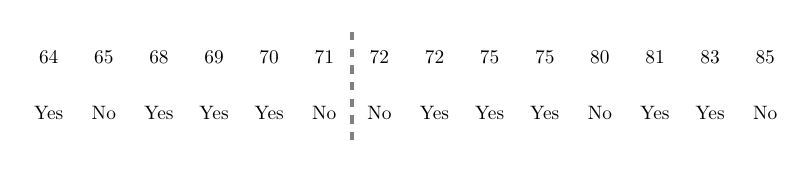
\begin{tikzpicture}[
		scale=0.7,
		every node/.style={scale=0.7}
	]

		\foreach \x/\v/\l in {
			1/64/Yes,2/65/No,3/68/Yes,4/69/Yes,5/70/Yes,6/71/No,7/72/No,
			8/72/Yes,9/75/Yes,10/75/Yes,11/80/No,12/81/Yes,13/83/Yes,14/85/No}{
			\node at (\x, 0) {\highlight{\v}};
			\node at (\x, -1) {\highlight{\l}};
		}

		\draw[gray,dashed,ultra thick] (6.5,-1.5) -- (6.5,0.5);
		
	\end{tikzpicture}
\end{figure}
	\divideTwo{0.49}{
		\begin{itemize}
			\item $\texttt{Temperature} < 71.5$ \\
				{\footnotesize yes: 4 | no: 2}
		\end{itemize}
	}{0.49}{
		\begin{itemize}
			\item $\texttt{Temperature} \ge 71.5$ \\
				{\footnotesize yes: 5 | no: 3}
		\end{itemize}
	}
	\vspace*{2mm}
	\begin{equation*}
			E(\mathcal{D}, \texttt{Temp.})
				= \nicefrac{6}{14} \cdot E(\texttt{Temp.} < 71.5) + \nicefrac{8}{14} \cdot E(\texttt{Temp.} \ge 71.5)
				= \bm{0.939}
		\end{equation*}
\end{frame}


% Handling numeric Attributes (Ctd.)
\begin{frame}{Handling numeric Attributes (Ctd.)}{}
	\begin{table}[h]
	\scalebox{0.95}{
		\begin{tabular}{| c | c | c | c | c | c | c | c | c | c |}
			\hline
			\multicolumn{10}{| c |}{\textbf{Sorted Values}} \\ \hline\hline
			\cellcolor{lightgray}{No} &
			\cellcolor{lightgray}{No} &
			\cellcolor{lightgray}{No} &
			\cellcolor{myblue2}{Yes} &
			\cellcolor{myblue2}{Yes} &
			\cellcolor{myblue2}{Yes} &
			\cellcolor{lightgray}{No} &
			\cellcolor{lightgray}{No} &
			\cellcolor{lightgray}{No} &
			\cellcolor{lightgray}{No} \\ \hline
			\multicolumn{10}{| c |}{\textbf{Taxable Income}} \\ \hline
			60 & 70 & 75 & 85 & 90 & 95 & 100 & 120 & 125 & 220 \\ \hline
		\end{tabular}
	}
\end{table}

\vspace*{-3mm}
{
	\renewcommand{\arraystretch}{1.5}
		\begin{table}[h]
			\scalebox{0.65}{
				\begin{tabular}{| l || c | c | c | c | c | c | c | c | c | c | c | c | c | c | c | c | c | c | c | c | c | c |}
					\hline
					Split &
					\multicolumn{2}{ c |}{55} &
					\multicolumn{2}{ c |}{65} &
					\multicolumn{2}{ c |}{72} &
					\multicolumn{2}{ c |}{80} &
					\multicolumn{2}{ c |}{87} &
					\multicolumn{2}{ c |}{92} &
					\multicolumn{2}{ c |}{97} &
					\multicolumn{2}{ c |}{110} &
					\multicolumn{2}{ c |}{122} &
					\multicolumn{2}{ c |}{172} &
					\multicolumn{2}{ c |}{230} \\ \hline
					
					& $\le$ & $>$ & $\le$ & $>$ & $\le$ & $>$ & $\le$ & $>$ & $\le$ & $>$ & $\le$ & $>$ &
					$\le$ & $>$ & $\le$ & $>$ & $\le$ & $>$ & $\le$ & $>$ & $\le$ & $>$ \\ \hline

					\cellcolor{myblue2}{Yes} &
					0 & 3 & 0 & 3 & 0 & 3 & 0 & 3 & 1 & 2 & 2 & 1 & 3 &
					0 & 3 & 0 & 3 & 0 & 3 & 0 & 3 & 0 \\ \hline
					\cellcolor{lightgray}{No} &
					0 & 7 & 1 & 6 & 2 & 5 & 3 & 4 & 3 & 4 & 3 & 4 & 3 &
					4 & 4 & 3 & 5 & 2 & 6 & 1 & 7 & 0 \\ \hline\hline
					\highlight{Gini} &
					\multicolumn{2}{ c |}{\highlight{0.420}} &
					\multicolumn{2}{ c |}{\highlight{0.400}} &
					\multicolumn{2}{ c |}{\highlight{0.375}} &
					\multicolumn{2}{ c |}{\highlight{0.343}} &
					\multicolumn{2}{ c |}{\highlight{0.417}} &
					\multicolumn{2}{ c |}{\highlight{0.400}} &
					\multicolumn{2}{ c |}{\highlight{\underline{0.300}}} &
					\multicolumn{2}{ c |}{\highlight{0.343}} &
					\multicolumn{2}{ c |}{\highlight{0.375}} &
					\multicolumn{2}{ c |}{\highlight{0.400}} &
					\multicolumn{2}{ c |}{\highlight{0.420}} \\ \hline
			\end{tabular}
		}
	\end{table}
}
\end{frame}


% Regression Trees
\begin{frame}{Regression Trees}{}
	\begin{itemize}
		\item Prediction of continuous variables
		\item Predict average value of all examples in the leaf
		\item Split the data such that variance in the leaves is minimized
		\item \textbf{Termination criterion is important, otherwise single point per leaf!}
	\end{itemize}
	\begin{boxBlueNoFrame}
		\highlight{Standard deviation reduction (SDR):}
		\begin{equation}
			SDR(\mathcal{D}, \texttt{A}) = SD(\mathcal{D})
				- \sum_{v \in dom(\texttt{A})} \frac{\vert \mathcal{D}_{\texttt{A}=v} \vert}{\vert \mathcal{D} \vert}
				\cdot SD(\mathcal{D}_{\texttt{A}=v})
		\end{equation}
	\end{boxBlueNoFrame}
\end{frame}


% Introduction Ensemble Methods
\begin{frame}{Introduction Ensemble Methods}{}
	\begin{itemize}
		\item \textbf{Key Idea}: Don't learn a single classifier but a \textbf{set of classifiers}
		\item Combine the predictions of the single classifiers to obtain the final prediction
	\end{itemize}
		
	\begin{boxBlue}
		\footnotesize
		\highlight{Problem:} How can we induce multiple classifiers from a single data set without getting
		the same classifier over and over again? \textbf{We want to have diverse classifiers,
		otherwise the ensemble is useless!}	
	\end{boxBlue}
		
	\begin{itemize}
		\item Basic techniques:
		\begin{itemize}
			\item \highlight{Bagging}
			\item \highlight{Boosting}
			\item \highlight{Stacking}
		\end{itemize}
	\end{itemize}
\end{frame}


% What is the Advantage?
\begin{frame}{What is the Advantage?}{}
	\begin{itemize}
		\item Consider the following:
		\begin{itemize}
			\item There are 25 \textbf{independent} base classifiers
			\item \highlight{Independence assumption:}
				Probability of misclassification \textbf{does not} depend on other classifiers in the ensemble
			\item Usually, this assumption does not fully hold in practice
			\item Each classifier has an error rate of $\epsilon = 0.35$
		\end{itemize}
		\item The ensemble makes a wrong prediction \textbf{if the majority is wrong} \\
			($\Rightarrow$ i.\,e. at least 13)
		\begin{equation}
			\epsilon_{ensemble}
				= \sum_{i=13}^{25} \binom{25}{i} \cdot \epsilon^i \cdot (1 - \epsilon)^{25 - i}
				\approx \bm{0.06 \ll \epsilon}
		\end{equation}
	\end{itemize}
\end{frame}


% Bagging
\begin{frame}{Bagging: General Approach}{}
	Bagging $\widehat{=}$ \highlight{B}ootstrap \highlight{Agg}regat\highlight{ing}
	\vspace*{-2mm}
	\begin{figure}
	\centering
	\begin{tikzpicture}[
		scale=0.28,
		custCylinder/.style={
			cylinder,draw=black,thick,aspect=0.7,minimum height=1.0cm,minimum width=0.7cm,shape border rotate=90,
			cylinder uses custom fill, cylinder body fill=myblue1!70,cylinder end fill=myblue1!30
		},
		arrow/.style={
			shorten >=0.5mm,shorten <=0.5mm,->,thick
		},
		dia/.style={
			diamond,draw=black,fill=lightgray,thick
		}
	]
	
		\node[custCylinder] (D) at (0,0) {\tiny $\mathcal{D}$};
		\node[custCylinder] (D1) at (-12,-5) {\tiny $\mathcal{D}_1$};
		\node[custCylinder] (D2) at (-6,-5) {\tiny $\mathcal{D}_2$};
		\node[custCylinder] (D3) at (0,-5) {\tiny $\mathcal{D}_3$};
		\node[custCylinder] (D4) at (12,-5) {\tiny $\mathcal{D}_k$};
		\node (D5) at (6,-5) {\tiny \textbf{...}};

		\draw[arrow] (D) -- ++(-12,0) -- (D1);
		\draw[arrow] (D) -- (D2);
		\draw[arrow] (D) -- (D3);
		\draw[arrow] (D) -- ++(12,0) -- (D4);
		\draw[arrow,dashed] (D) -- (D5);

		\node[dia] (C1) at (-12,-10) {\tiny $\bm{C}_1$};
		\node[dia] (C2) at (-6,-10) {\tiny $\bm{C}_2$};
		\node[dia] (C3) at (0,-10) {\tiny $\bm{C}_3$};
		\node[dia] (C4) at (12,-10) {\tiny $\bm{C}_k$};
		\node (C5) at (6,-10) {\tiny \textbf{...}};

		\draw[arrow] (D1) -- (C1);
		\draw[arrow] (D2) -- (C2);
		\draw[arrow] (D3) -- (C3);
		\draw[arrow] (D4) -- (C4);
		\draw[arrow,dashed] (D5) -- (C5);

		\node[star,star points=7,star point ratio=0.8,draw=black,fill=yellow!30] (E) at (0,-15) {\tiny $\bm{C^*}$};
		\draw[arrow] (C1) -- ++(0,-5) -- (E);
		\draw[arrow] (C2) -- (E);
		\draw[arrow] (C3) -- (E);
		\draw[arrow] (C4) -- ++(0,-5) -- (E);
		\draw[arrow,dashed] (C5) -- (E);

		\node[align=center] at (-20,-5) {\footnotesize Create \\[-2mm] \footnotesize multiple data sets};
		\node[align=center] at (-20,-10) {\footnotesize Build \\[-2mm] \footnotesize multiple classifiers};
		\node[align=center] at (-20,-15) {\footnotesize Combine decisions};
		
	\end{tikzpicture}
\end{figure}
\end{frame}


% Creating the Bootstrap Samples
\begin{frame}{Creating the Bootstrap Samples}{}
	\begin{itemize}
		\item How to generate multiple data sets which are different?
		\item \textbf{Solution:} Use sampling with replacement
		\vspace*{2mm}
		\begin{table}[h]
	\scalebox{0.8}{
		\begin{tabular}{| l || c | c | c | c | c | c | c | c | c | c |}
			\hline
			\cellcolor{myblue1!70}{\textbf{Original Data}}	
				&	1 	&	2	&	3	&	4	&	5	&	6	&	7	&	8	&	9	&	10
			\\ \hline
			\cellcolor{myblue1!70}{\textbf{Bagging (Round 1)}}
				&	7 	&	8	&	10	&	8	&	2	&	5	&	10	&	10	&	5	&	9 
			\\ \hline
			\cellcolor{myblue1!70}{\textbf{Bagging (Round 2)}}
				&	1 	&	4	&	9	&	1	&	2	&	3	&	2	&	7	&	3	&	2
			\\ \hline
			\cellcolor{myblue1!70}{\textbf{Bagging (Round 3)}}
				&	1 	&	8	&	5	&	10	&	5	&	5	&	9	&	6	&	3	&	7
			\\ \hline
		\end{tabular}
	}
\end{table}
		\vspace*{2mm}
		\item Some examples may appear \textbf{in more than one set}
		\item Some examples may appear \textbf{more than once} in one set
		\item Some examples may \textbf{not appear at all}
	\end{itemize}
\end{frame}


% Bagging Algorithm
\begin{frame}[plain]{}{}
	\begin{algorithm}[H]
		\setstretch{1.4}
		\DontPrintSemicolon
		\footnotesize
		\KwIn{Training set $\mathcal{D}$, number of base classifiers $n$}
		\highlight{Training:}\;
		\ForAll{$i \in \{ 1, 2, \dots, k \}$}{
			Draw a bootstrap sample $\mathcal{D}_i$ with replacement from $\mathcal{D}$\;
			Learn a classifier $C_i$ from $\mathcal{D}_i$\;
			Add classifier $C_i$ to the ensemble\;
		}
		\highlight{Prediction:}\;
		\ForAll{unlabeled instances}{
			Get predictions from all classifiers $C_i$\;
		}
		\Return{Class which receives the majority of votes (combined classifier $C^*$)}
 		\caption{Bagging Algorithm}
	\end{algorithm}
\end{frame}


% Bagging Variations
\begin{frame}{Bagging Variations}{}
	\begin{itemize}
		\item The bootstrap samples had equal size and were drawn with replacement
		\item Also conceivable:
		\begin{enumerate}
			\item \textbf{Varying the size} of the bootstrap samples
			\item Sampling \textbf{without replacement} $\Rightarrow$ \highlight{Pasting}
			\item \textbf{Sampling of features}, not instances
			\begin{itemize}
				\item Not all features are available in all bootstrap samples
				\item This is how \highlight{random forests} work
			\end{itemize}
			\item Creating \textbf{heterogeneous ensembles} \\
				(Neural networks, decision trees, support vector machines, ...)
		\end{enumerate}
	\end{itemize}
\end{frame}


% Section: Wrap-Up
%______________________________________________________________________
\section{Wrap-Up}
\makedivider{Wrap-Up}

% Subsection: Summary
% --------------------------------------------------------------------------------------------------------
\subsection{Summary}

% Summary
\begin{frame}{Summary}{}

\end{frame}


% Subsection: Lecture Overview
% --------------------------------------------------------------------------------------------------------
\subsection{Lecture Overview}

\makeoverview{3}


% Subsection: Self-Test Questions
% --------------------------------------------------------------------------------------------------------
\subsection{Self-Test Questions}

% Self-Test Questions
\begin{frame}{Self-Test Questions}{}

\end{frame}


% Subsection: Recommended Literature and further Reading
% --------------------------------------------------------------------------------------------------------
\subsection{Recommended Literature and further Reading}

% Literature
%______________________________________________________________________
\begin{frame}{Recommended Literature and further Reading}{}
	\footnotesize
	\begin{thebibliography}{2}

	\end{thebibliography}
\end{frame}


% Thank you
%______________________________________________________________________
\makethanks

\end{document}